% Just realized: b/c of anonymity, the PC can't chastise us for
% running our system on our own code -- we can't tell them that it's our code!

\colin{Should discuss fidelity of log messages (distinguish different failure
modes) and what we want (ODR) here}

\colin{
Logical clocks don't work for all situations! Consider a link failure that
is detected by both adjacent switches connected to the link. Which one
observed the link failure first? The message "link went down" doesn't include
a logical clock...
}

\colin{WRT snapshotting:
we assume that network hardware has the primitives necessary to support a
causally-consistent snapshot algorithm (viz. transactional queries to the
FIB/RIB).}

\colin{WRT fidelity: make the point that we can always
increase the fidelity of the simulator -- it's all just software}

\colin{TODO: paragraph on how this approach might apply to traditional
networks}

We now discuss the overhead of using \simulator{} in a production environment,
detail scalability properties of our system, and discuss how the assumptions
detailed in Section~\ref{sec:approach} can be relaxed.

\subsection{Overhead}

\noindent{\bf Network Snapshot Overhead:} In contrast to general record-and-replay
mechanisms, the amount of recorded state needed for
high-fidelity replay is tractable\andi{Check with our newly, well defined strong assumptions: 
we need full internal/external events. Is this tractable}. With proactive flow installation,
updates are pushed to routing tables over a relatively long time scale; periodic
FIB snapshots along with a log of link state events, control server
downtime, host mobility information, and policy-changes suffice for our purposes.
Assuming a maximum of 256K routing or ACL entries per switch~\cite{cisco7000}, and 
36 bytes per entry, each FIB will contain a maximum of 9216
kilobytes, uncompressed. A fat tree network of 27,648 hosts
includes 2,880
switches~\cite{Al-Fares:2008:SCD:1402958.1402967}.
Therefore a snapshot of the FIBs of the entire network would naively take up roughly
26 GB. Note however, that the data is likely to be compressible quite well, due to do its
structural and temporal properties. Assuming 8.5 error events per minute per
datacenter~\cite{Greenberg:2009:VSF:1592568.1592576}, 1,000,000
VM placement changes per day per datacenter~\cite{Soundararajan:2010:CBS:1899928.1899941},
and a small rate of human-specified policy changes, the log of the external inputs
should grow at a rate of \textasciitilde 750 entries per minute.

%To account for host mobility, assume that each server hosts 10 VMs,
%and 1\% of VMs are created, suspended, or migrated every minute. Then 10,000 host mobility events must be
%logged per minute, also a reasonable storage cost.

\eat{
\colin{Notes from Rean Griffith:
\begin{itemize}
\item total vms in a typical datacenter: 1000
\item migration frequency (migrations/minute): 20 per hour
\item VM spin ups/downs: 150 power ons per hour (see our OSR 2010 paper for
power off estimates)
\item Do we log VM migrations and how does that log grow (I wasn't able to
get any estimates on log-growth data)
\end{itemize}

We had an OSR 2010 paper that provided numbers scaled by the number of
VMs in an installation:
Challenges in building scalable virtualized datacenter management
(http://dl.acm.org/citation.cfm?id=1899941)
}
}

%As a point of reference, border routers' working RIB size is
%$\textasciitilde$130MB~\cite{Karpilovsky:2006:UFR:1368436.1368439}.
\eat{

TODO: Replace this analysis.
It stinks. PORTLAND is not the right way to evaluate this due to the lacking number of rules.

\noindent{\bf Correspondence Checking Runtime.} 
Computing the propagation
graph for correspondence checking is equivalent to enumerating
all possible paths in the network, which scales with the diameter
of the network and the number of routing entries per switch.
The propagation graph for each host can be
computed in parallel however, so the computation is bottlenecked by the serial runtime
of computing a single host's propagation graph.

We show the serial runtime of correspondence checking in
Figure~\ref{fig:hsa_runtime}. For this analysis we generated fat tree topologies
between 2 and 48 pods wide, with pre-installed PORTLAND~\cite{NiranjanMysore:2009:PSF:1592568.1592575}
routing tables in each switch. Each data point is the minimum of three
runs on a single Intel Xeon 2.80GHz core. Note that the number of PORTLAND routing entries per switch scales with the number
of pods in the fat-tree. We excluded the time to convert
flow tables to HSA transfer functions, since transfer functions can be maintained
offline.

As the figure depicts, even for large networks
(27,648 hosts) the serial runtime of correspondence checking is reasonable for
interactive use. The number of serial tasks to be executed
is the number of hosts in the network squared, disregarding ECMP load balancing.

\begin{figure}[t]
    %\hspace{-10pt}
    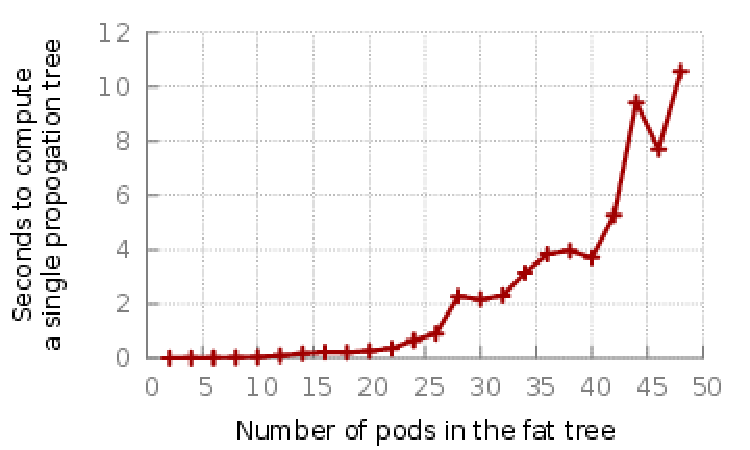
\includegraphics[width=3.25in]{../graphs/hsa_overhead_graph/graph.pdf}
    \caption[]{\label{fig:hsa_runtime} Serial runtime of correspondence
    checking on PORTLAND fat tree networks. Each datapoint consists of
    $x^3/4$ hosts and $5x^2/4$ switches (\eg{} 48 pods means 27,468 hosts
    attached to 2,880 switches)}
\end{figure}
}

\eat{ This evaluation stinks. Be gone!

\noindent{\bf Simulator Scalability.} As our approach depends on the frequently
repeating simulations, we now evaluate the setup time incurred by the simulator
system when handling large network topologies. For this experiment, shown in
Figure~\ref{fig:scalability}, we generate fat tree topologies between 2 and 48
pods wide, where all switches in the network connected to a single controller.
The controller sends each switch an OpenFlow $FLOW\_MOD$ and subsequent
$BARRIER\_REQUEST$ message, and waits for the corresponding $BARRIER\_REPLY$. We
then measure the time to between the first $FLOW\_MOD$ sent and the last
$BARRIER\_REPLY$ received. As expected, the runtime was roughly linear with the
number of switches in the network. The figure also shows that the processing
time for large networks (5 seconds per simulator round) was well within the
bounds for interactive use.

\begin{figure}[t]
    %\hspace{-10pt}
    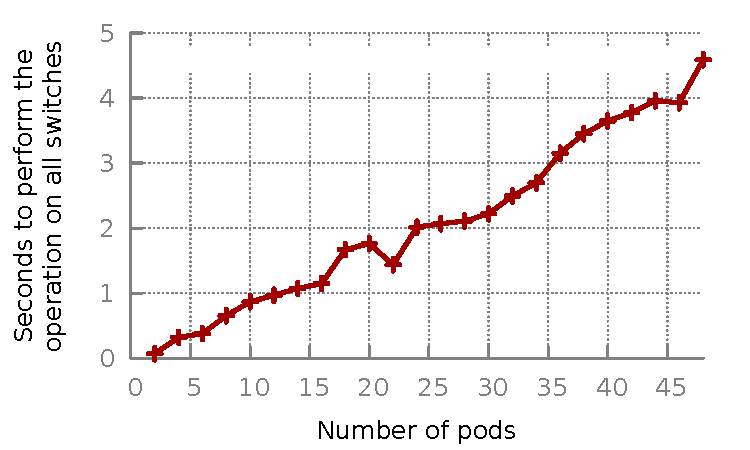
\includegraphics[width=3.25in]{../graphs/scalability_graph/scale.pdf}
    \caption[]{\label{fig:scalability} Time to send and process messages
    between controller and simulated switches. Each datapoint consists of
    $x^3/4$ hosts and $5x^2/4$ switches (\eg{} 48 pods means 27,468 hosts
    attached to 2,880 switches)}
\end{figure}

We also tested the extreme limits of the simulator's scalability, pushing up
the number of switches until something broke. We encountered what appears to be
a limitation of the Linux TCP/IP stack: TCP connection attempts began failing
beyond 26,680 sockets. Note that 26,680 switches is an order-of-magnitude larger than
the today's biggest networks.
}

\subsection{Simulation fidelity}

On the one hand, since the SDN platform is in software, we can, in theory,
reproduce all software-induced policy violations (though not problems
resulting from flaky hardware implementing code incorrectly). However, this
requires setting up the simulator to emulate the appropriate conditions that
led to the policy violation, and that can be quite difficult. We hope to make
progress in this area along two dimensions.  First, we hope to help the
community build up a set of regression tests, so that a wide variety of
bug-triggering scenarios are available in a public repository. This would go a
long way towards providing adequate test coverage.

Second, we hope to gather error logs from real production deployments which
will help us populate this repository; this may require providing novel kinds
of anonymization, so that large datacenter operators would be willing to share
their problems (since they want their SDN code to work) without revealing the
details of their network.  This may require a infrastructural counterpart to
minimally-causal events; the smallest number of infrastructure components that
can reproduce the same bug.


\colin{TODO: add note about not being able to tell difference between
endogenous and exogenous events, which might hide the true cause of a bug.
This is OK though, since we assume that the platform should always have a
correct option, but it doesn't take it. That is, the root cause of the crash
is not what we're interested in (software vs. hardware), it's how the platform
reacts to that crash that matters (should be robust, no matter what the
cause of the crash)}

\colin{Note that we also assume an out-of-band management network between
switches and controllers, and that the management network always provides 
connectivity. We could add the management network into our model if we want, I
suppose.}
